% !TeX spellcheck = en-GB
\section{Materials \& Methods}
The automatic segmentation evolves around a Random Forest classifier. In \autoref{fig:pipeline} the whole segmentation pipeline is shown. The individual parts of the segmentation are covered in the following subsections. Furthermore the validation of the automatic segmentation is described.

To train the RF and evaluate the performance of the segmentation two data sets are used. The first data set comprises 20 MRI volumes and their ground truth. This data set is used to train the RF and evaluate quantitative the segmentation. The second data set contains 10 MRI volumes without ground truth, which are used to evaluate the segmentation qualitative.
\subsection{Pre processing}
In order to compensate for different MRI grey-scale representations, the images are normalized using z-score normalisation (\autoref{eq:zscorenormalize}). In a second step a Wiener filter is applied to reduce noise. This yields a normalized representation of the data, that is used for the next steps.
\begin{equation}
I_n = \frac{I - \mu}{\sigma}
\label{eq:zscorenormalize}
\end{equation}
\subsection{Feature Extraction \& Random Forest}
Thirteen different features are extracted for each voxel of the normalized data, which are used to apply the RF. The features cover different aspects of the data. To describe vertical and horizontal edges we use Prewitt and Sobel. The derivatives are covered by Laplacian and Laplacian of Gaussian and the intensity by Gaussian and Average filters. The statistical information is represented by the entropy and the standard deviation features. To restrict the classifier to the femur we added the relative position in 3D, with the assumption that the femur rotates and moves only slightly between the different MRI volumes. To compensate for different image resolutions the relative position is used instead of the absolute.

The RF tree model is created by training a RF with 15 trees on 1\% of the voxels from the training images, which are randomly picked. Applying the RF tree model on the extracted features yields the segmented femur.
%We used 13 different features of which we had edge representations like Prewitt and Sobel, derivatives using the Laplacian and Laplacian of Gaussian and intensity information using Gaussian and Average filters. Additionally we added statistical information entropy and standard deviation. To restrict the classifier to the Femur, we added the relative position in 3D. The relative position is used instead of the absolute, to compensate for different image resolutions.
%The RF classifier is trained using 15 trees and 1\% of the voxels from the training images, which are randomly picked. 
\subsection{Post processing}
After the prediction of the Random Forest classifier, the results are post processed to remove outliers. The implemented post processing comprises following four steps, where the 2D operations are applied on each slice and the 3D operation on the volume:
\begin{enumerate}
\item 2D Morphological opening
\item 2D Keep largest area
\item 2D Morphological filling
\item 3D Keep largest volume
\end{enumerate}
Applying this four steps yields the final segmented volume. In order to present the result, the volume is converted to a mesh by applying a marching cubes algorithm. 
\subsection{Validation}
To validate the whole segmentation, a randomized 5-fold cross validation \cite{cross} is used on the first data set. Out of the 20 volumes 16 are used to train and 4 to test the algorithm. To measure the accuracy and robustness the mean DICE coefficient and the standard deviation over all 20 results is used.
\begin{figure*}[!t]
\centering
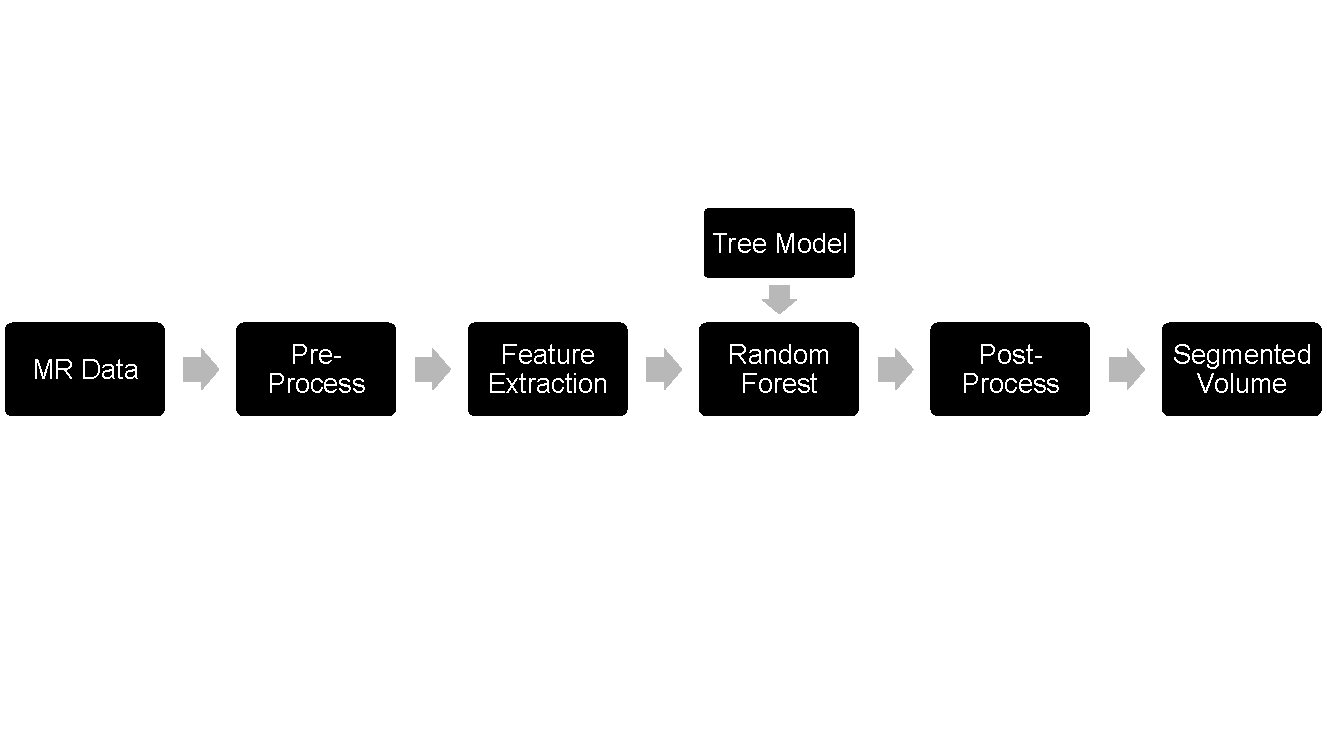
\includegraphics[width=\textwidth]{pipeline}
\caption{Pipeline of the automatic segmentation using a trained Random Forest model to segment the femur from MRI data.}
\label{fig:pipeline}
\end{figure*}

%fully automatic
%show the pipeline
%preprocessing (normlization, wiener filer), maybe show picture
%training, features, relative position, show kernels, number of trees, 2d features
%postprocessing, opening, largest area, filling, largest volume, show images as in presentation
%explain our cross validation procedure (DICE not OOB score)
